\chapter{Desarrollo software del manipulador}
\label{cap:capitulo6}

\vspace{1cm}
\noindent En este capítulo se aborda el desarrollo software necesario para poder usar el robot realizado 
tanto en simulaciones como en el mundo real.

\section{Control de los actuadores}

En robótica, los actuadores son los componentes responsables de convertir las señales eléctricas 
en movimiento físico.

Para realizar el control de los actuadores se ha optado por utilizar el firmware de control numérico 
GRBL\ref{subsec:grbl}. Se ha optado por el uso de este firmware por encima de realizar uno propio, 
debido a que es una solución robusta con años de desarrollo y una comunidad que lo respalda.

Este firmware, permite controlar hasta 3 motores paso a paso simultáneamente. Además está optimizado para ejecutarse en 
microcontroladores de bajos recursos y hace uso de herramientas hardware de bajo nivel, como los \textit{timers} o los 
contadores para garantizar una operación fiable.

Para que GRBL sepa qué posición debe tener cada motor en un momento dado, necesita recibir 
una serie de datos codificados a través de una de sus interfaces. Los detalles de la comunicación 
serán descritos en la siguiente sección.

\section{Comunicación con el robot}
En esta sección se exponen los mecanismos necesarios para permitir la comunicación entre el ordenador y 
el microcontrolador alojado en la base del robot, así como, la arquitectura del sistema robótico. Además se detallan las configuraciones necesarias 
para adaptar al mundo de la robótica las diferentes partes que lo componen.

En base a las especificaciones del manual\footnote{\url{https://raw.githubusercontent.com/makerbase-mks/MKS-DLC32/main/doc/DLC32\%20wiring\%20manual.pdf}} 
de la placa, permite establecer comunicaciones via USB serie y existe la posibilidad (reside en el propio firmware) de utilizar la funcionalidad 
Wi-Fi del ESP32. 
La comunicación obtenida mediante el uso del puerto USB se realiza sobre el protocolo \ac{UART}. Este protocolo serie es utilizado para 
transmitir datos de forma asíncrona entre dispositivos. Es comúnmente usado en la interconexión de microcontroladores, 
periféricos y otros componentes electrónicos. El UART convierte los datos paralelos en datos serie y viceversa, utilizando bits 
de inicio, datos, bits de parada y posiblemente bits de paridad para la sincronización y detección de errores. 
\begin{figure} [h!]
    \begin{center}
    \includegraphics[width=12cm]{figs/uart.png}
    \end{center}
    \caption{Diagramas de tiempo de UART}
    \label{fig:uart}
\end{figure}\ 
Otra forma de comunicarnos con la placa es mediante el uso del su adaptador inalámbrico Wi-Fi. Existen firmwares, como es el caso de 
Grbl, que tienen una versión adaptada para microcontroladores con conectividad Wi-Fi que permiten enviar comandos usando una gran 
variedad de protocolos convencionales usados en redes de ordenadores. En este caso, Telnet. 

Además, el firmware de Grbl es capaz de levantar un punto de acceso inalámbrico al cual puedes conectarte como si de un router 
se tratara y se puede acceder a un servidor alojado en su dirección IP. Para acceder a él, basta con introducir 192.168.1.1 en la 
barra superior del navegador web para acceder a una interfaz de usuario que permite controlar los movimientos de la máquina. En este 
caso tiene un aspecto peculiar y no amigable con el mundo de la robótica ya que está pensado para el uso en CNC. Es por esto que es 
necesario realizar unas ciertas configuraciones para su uso en robótica.

grbl wifi
grbl cable
biblioteca python usada
detalles de la comunicacion via codigo G
ejemplos de uso ugs 


\subsection{Adaptación de grbl para su uso en robótica}
GRBL tiene ciertas limitaciones a la hora de su utilización en robótica. Es normal, debido a que está pensado para controlar máquinas 
\acs{CNC} de 3 ejes prismáticos. Pese a esto, se pueden hacer ciertas modificaciones para adaptarlo a esta aplicación. 

\subsubsection{Parámetros de Grbl}
Para acceder y modificar los parámetros de Grbl se deben realizar los siguientes pasos:
\begin{enumerate}
\item Debemos tener conectada al ordenador la placa con el firmware de Grbl instalado.
\item Podemos usar un programa especializado con interfaz gráfica como \ac{UGS} o mediante una terminal serial, como puede ser Cutecom.
\item Introducimos la velocidad de trasmisión de Grbl por defecto; 115200 baudios. 
\item Para preguntar al firmware sobre los parámetros que hay configurados, introducimos los caracteres: \$\$
\item Para modificar un parámetro, introducimos un texto del estilo: \$número=nuevoValor
\end{enumerate}

Para su uso en robótica nos interesa modificar los siguientes parámetros: 
\begin{itemize}
\item \textbf{\$1}: Retardo o tiempo de espera entre pulsos de paso cuando el motor está inactivo (en milisegundos). Debemos configurar 
este parámetro en su valor máximo, en este caso 255. Este valor tiene un significado especial, haciendo que los motores paso a paso 
se mantendrán energizados constantemente aunque no se estén moviendo. Es de vital importancia para evitar que el brazo se desplome tras terminar un cierto movimiento.  
\item \textbf{\$100}, \textbf{\$101} y \textbf{\$102}: Indican el número de pasos por unidad de movimiento para los ejes X, Y, Z respectivamente. 
\\Por defecto está pensado para utilizar pasos por milímetro. Como se pretende utilizar articulaciones de rotación, debemos expresar esta relación 
en función de alguna medida angular. La unidad a utilizar podría ser: grados, radianes o vueltas, entre otras. En este trabajo se 
utilizan los grados debido a que en radianes y vueltas la unidad correspondía a un gran número de pasos y era dificil controlar la aceleración para incrementos de 
0.1 vueltas. 

\begin{myequation}[h!]
\begin{equation}
    PasosPorGrado = \frac{Microstepping * Ratio}{1.8^\circ}
\nonumber
\label{ec:pasos_por_grado}
\end{equation}
\caption[Cálculo de pasos por grado en Grbl]{Cálculo de pasos por grado en Grbl}
\end{myequation} 

\item \textbf{\$110}, \textbf{\$111} y \textbf{\$112}: Indican la velocida máxima a la que puede moverse cada eje X, Y, Z en "unidades" por segundo. 
En este caso, grados por segundo. Estos valores se deben encontrar por medio de la experimentación. Se trata de una medida de seguridad en 
caso de que el usuario quiera mover demasiado rápido un eje pudiendo dañar el brazo.

\item \textbf{\$120}, \textbf{\$121} y \textbf{\$122}: Indican la aceleración máxima a la que puede moverse cada eje X, Y, Z en "unidades" por segundo cuadrado. 
En este caso, grados por segundo cuadrado. Estos valores tambien se deben encontrar por medio de la experimentación. Se trata de una medida de seguridad en 
caso de que el usuario quiera mover demasiado rápido un eje pudiendo dañar el brazo. Se debe encontrar una aceleración idónea para todos 
los movimientos, una limitación de grbl es que no se puede comandar un movimiento diciendole una determinada aceleración.

\end{itemize}

\begin{table}[H]
\begin{center}
\begin{tabular}{|c|c|}
\hline
\textbf{Parámetro} & \textbf{Valor} \\
\hline
\$0 & 0 \\
\$1 & 255 \\
\$2 & Bla \\
\$0 & 0 \\
\$0 & 0 \\
\$0 & 0 \\
\$0 & 0 \\

\end{tabular}
\caption{Parámetros Grbl usados en este trabajo}
\label{cuadro:parametros_grbl}
\end{center}
\end{table}

En esta página oficial de documentación se profundiza más en la finalidad de cada parámetro.
Para mas info: https://github.com/gnea/grbl/blob/master/doc/markdown/commands.md

%26.\wideparen{6}\\
Para mas info: https://github.com/gnea/grbl/blob/master/doc/markdown/settings.md


\newpage
\section{Integración con ROS 2}
En esta sección se detalla el proceso de integración del robot G-Arm en \acs{ROS}.

\subsection{Descripción del robot}

\subsubsection{Creación del paquete de descripción}
\noindent Para crear el paquete, se ha seguido el siguiente
\begin{enumerate}
    \item Dentro de la carpeta \textit{src} del workspace ejecutamos:
    \begin{verbatim}
        ros2 pkg create --build-type ament_cmake g_arm_description
    \end{verbatim}   
    \item Dentro de la carpeta que se ha generado, creamos 3 nuevos directorios:
    \begin{verbatim}
        mkdir launch rviz urdf meshes
    \end{verbatim} 
        
    \item Añadimos al fichero \textit{package.xml}: 
        \lstset{
        language=XML, % Establece el lenguaje como XML
        basicstyle=\ttfamily, % Fuente monoespaciada
        keywordstyle=\bfseries\color{blue}, % Estilo de las palabras clave
        commentstyle=\itshape\color{gray}, % Estilo de los comentarios
        stringstyle=\color{orange}, % Estilo de las cadenas de texto
        showstringspaces=false, % No mostrar espacios en cadenas de texto
        breaklines=true, % Dividir líneas largas
        frame=lines, % Agregar un marco alrededor del código
        numbers=left, % Mostrar números de línea
        numberstyle=\tiny\color{gray}, % Estilo de los números de línea
        captionpos=b % Posición de la leyenda del código (abajo)
    }
    
    \begin{lstlisting}
        <buildtool_depend>ament_cmake</buildtool_depend>

        <exec_depend>joint_state_publisher</exec_depend>
        <exec_depend>robot_state_publisher</exec_depend>
        <exec_depend>rviz</exec_depend>
        <exec_depend>xacro</exec_depend>

        <test_depend>ament_lint_auto</test_depend>
    \end{lstlisting}
        
    \item Compilamos el paquete desde la raíz del workspace:
    \begin{verbatim}
        colcon build --symlink-install
    \end{verbatim}
    \item Añadimos la siguiente línea al final del .bashrc para que ROS pueda encontrar el paquete:
    \begin{verbatim}
        source ~/workspace/install/local_setup.bash
    \end{verbatim}
    
    \end{enumerate}

\subsubsection{Describir un robot mediante \ac{URDF} y Xacro}
Es un formato de archivo cuyo propósito es describir la estructura, cinemática y aspecto de un robot.  
Se trata de un estándar ampliamente utilizado en la comunidad de robótica, especialmente en \ac{ROS}.

En un archivo URDF, se especifica la geometría del robot mediante la definición de partes (links) y articulaciones (joints). 
Cada parte se describe mediante su forma y tamaño, mientras que las articulaciones definen las restricciones de movimiento y las relaciones entre los enlaces.
Además de esto, un archivo URDF también puede incluir información sobre la masa y la inercia de los enlaces, así como como texturas y modelos 3D.

El formato URDF se basa en el lenguaje \ac{XML}, lo que permite describir el robot de una forma estructurada y legible. Con la descripción 
en URDF, los robots pueden ser simulados, visualizados y controlados.

Para crear un paquete para describir un robot en ros2 debemos de seguir el siguiente procedimiento:



poner un tree para ver como queda todo 
hablar de urdf y xacro
hablar de rviz y controladores





\newpage
\subsection{Integración en MoveIt 2}
\noindent En esta sección se enumeran y describen los pasos necesarios para, apartir de un paquete de descripción de un robot, generar 
un paquete de MoveIt.
\\
Antes de comenzar, debemos tener instalado MoveIt 2 para ROS Humble. Para ello, se ha seguido el proceso de 
instalación\footnote{\url{https://moveit.picknik.ai/main/doc/tutorials/getting_started/getting_started.html}} de la documentación.
\\

Para crear el paquete de MoveIt de este robot, se han llevado a cabo los siguientes pasos:
\begin{enumerate}
\item Lanzamos el asistente de configuración.
\begin{verbatim}
    ros2 launch moveit_setup_assistant setup_assistant.launch.py
\end{verbatim}
\item Pulsamos sobre \textbf{\textit{\guillemotleft Create New MoveIt Configuration Package\guillemotright}} y cargamos el URDF/Xacro del paquete de descripción 
del robot. Si el fichero es válido, aparecerán una serie de apartados a configuar en el lateral izquierdo del asistente. 
\item Comenzamos configurando la apartado \textbf{\textit{\guillemotleft Self-Collisions\guillemotright}}. Aquí se hace uso de la colisiones 
descritas anteriormente para generar una matriz de posibles colisiones que se pueden dar. Para ello, pulsamos sobre
\textbf{\textit{\guillemotleft Generate Collision Matrix\guillemotright}}.
\item Acto seguido se configura el apartado \textbf{\textit{\guillemotleft Planning Groups\guillemotright}}, donde se establecen los eslabones y articulaciones que serán consideradas 
a la hora de realizar la planificación. Para ello, pulsamos sobre \textbf{\textit{\guillemotleft Add Group\guillemotright}} y acto seguido 
le damos un nombre. Posteriormente, pulsamos sobre \textbf{\textit{\guillemotleft Add Kin. Chain\guillemotright}} y seleccionamos como 
eslabón base, el eslabón que irá unido al suelo, y como eslabón \textit{tip}, el extremo del robot. Entonces, guardamos los cambios. Ahora, 
se añaden todos los \textit{links} y \textit{joints} al grupo de planificación creado, dando en \textbf{\textit{\guillemotleft Edit Selected\guillemotright}} 

\item En el apartado \textbf{\textit{\guillemotleft Robot Poses\guillemotright}} se pueden configurar una serie de posiciones predeterminadas 
para poder usarse posteriormente cuando se necesiten. Por ejemplo, es recomendable crear al menos dos; una que haga de posición \textit{Home} 
(Posición cómoda para empezar a trabajar) y otra como posición de reposo (Posición que evita que el robot se desplome al cortar la electricidad).

\item Usamos el apartado \textbf{\textit{\guillemotleft End Effectors \guillemotright}} para configurar el extremo de nuestro robot como tal. Para ello, 
seleccionamos el eslabón del extremo y el grupo de planificación creado anteriormente. 

\item En \textbf{\textit{\guillemotleft Passive Joints\guillemotright}}, añadimos todos aquellas articulaciones que no sean grados de libertad, 
es decir, todas aquellas que no sean \textit{joint1, joint2 o joint3}.

\item En los apartados \textbf{\textit{\guillemotleft ROS 2 Controllers\guillemotright}} y 
\textbf{\textit{\guillemotleft MoveIt Controllers\guillemotright}}, añadimos automaticamente los controladores pulsando sobre el único botón que hay.

\item Finalmente rellenamos nuestra información personal en \textbf{\textit{\guillemotleft Author information\guillemotright}} y generamos el 
paquete en el \textit{src} del \textit{workspace}. Acto seguido, compilamos.
\end{enumerate}

A la hora de usar esta herramienta, se debe de tener en cuenta que a día de la publicación de este trabajo, existe un error en el asistente
que hace que el paquete no se cree bien del todo. Para corregirlo, es necesario cambiar todos los número del fichero \textit{joints\_limits.yaml}
del paquete generado a \textit{double}. Es decir, cambiar por ejemplo un ``200" por ``200.0".
\\

Para probar que ha salido todo bien, ejecutamos:
\begin{verbatim}
    ros2 launch g_arm_moveit demo.launch.py
\end{verbatim}
Si todo se ha configurado bien deberíamos ver algo parecido a lo mostrado en la Figura \ref{fig:moveit_demo}. Para comprobar que resuelve una trayectoria sin 
problema, podemos establecer dos posiciones aleatorias y ejecutar la trayectoria (Figura \ref{fig:moveit_trayectory_demo}).
\begin{figure} [ht!]
    \begin{center}
      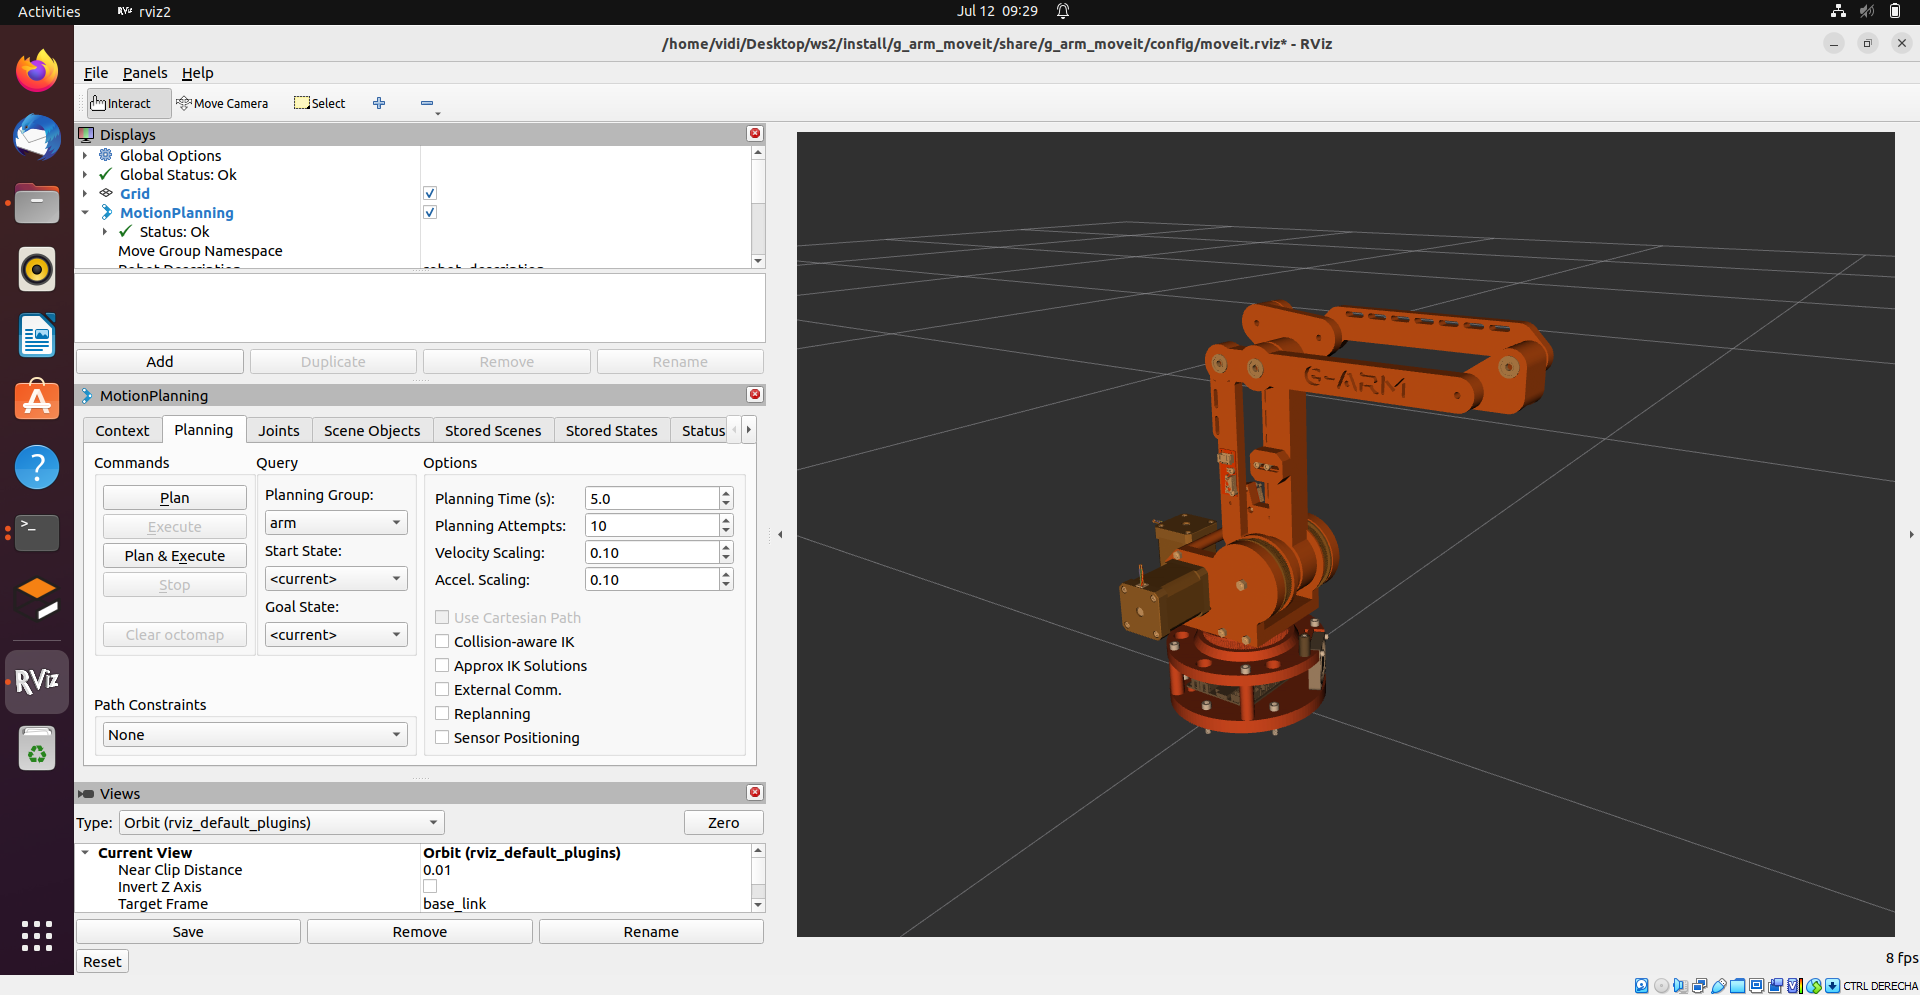
\includegraphics[width=15cm]{figs/moveit_demo.png}
    \end{center}
    \caption{Rviz al lanzar el \textit{demo.launch.py}}
    \label{fig:moveit_demo}
\end{figure}\ 

\begin{figure} [ht!]
    \begin{center}
      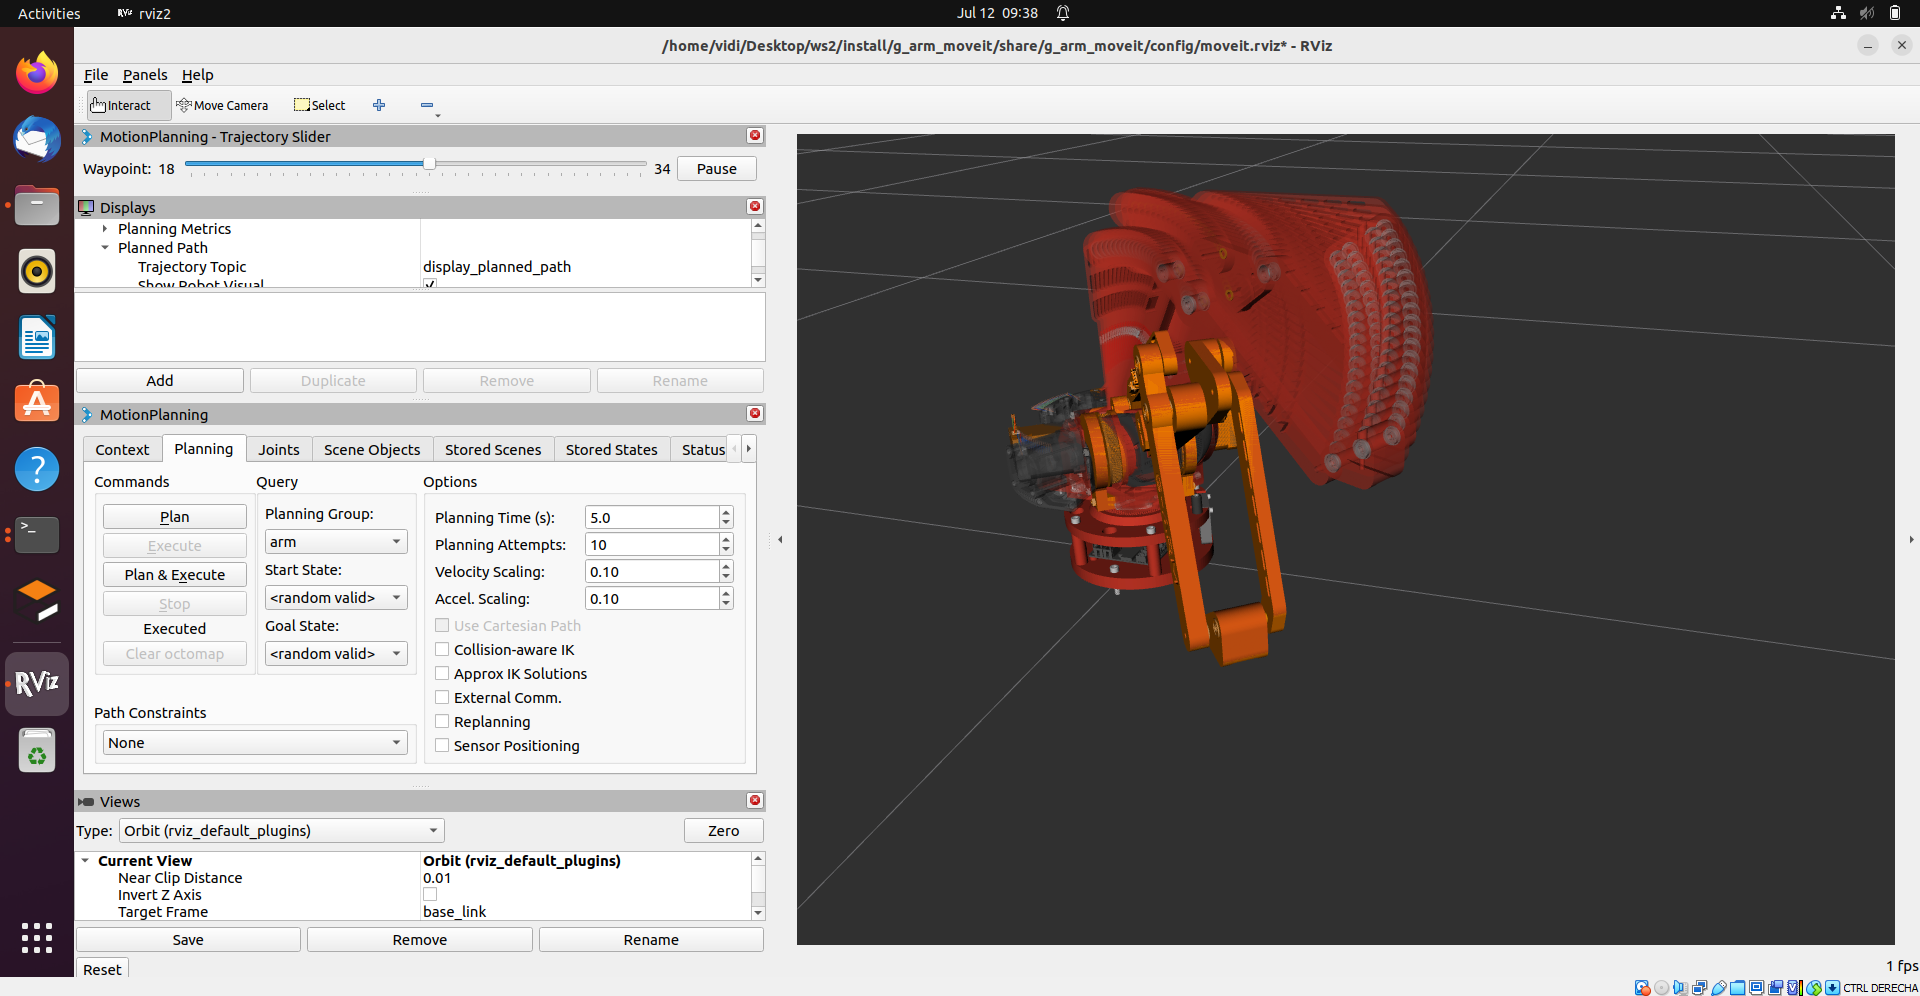
\includegraphics[width=15cm]{figs/moveit_demo_trajectory.png}
    \end{center}
    \caption{Planificando una trayectoria simple}
    \label{fig:moveit_trayectory_demo}
\end{figure}\ 
\\
\newpage
\subsection{Nodo ROS}
\noindent En esta sección se crea un nodo ROS capaz de interpretar los mensajes resultantes de MoveIt y mover el brazo real en función de ellos.
\\

Según la documentación\footnote{\url{https://moveit.picknik.ai/humble/doc/concepts/move_group.html}}, existe un nodo llamado 
\textit{move\_group} (Véase la Figura\ref{fig:arquitectura_moveit}) que se comunica con resto del framework 
a través de los \textit{topics} y acciones de ROS. Además, se comunica con el robot para obtener información acerca del estado 
actual (posiciones de las articulaciones, etc.), para obtener nubes de puntos y otros datos de los sensores del 
robot, y para interactuar con sus controladores.

Principalmente hay que centrarse en un \textit{topic} y una acción de ROS 2. 

El \textit{topic} es \textit{/joint\_states}, el cual es publicado por el nodo que debemos de crear nosotros 
y es recibido por \textit{move\_group}. La acción es \textit{/arm\_controller/follow\_joint\_trajectory} (el controlador ha sido nombrado como 
arm\_controller por defecto). 

%moveit_simple_controller_manager Es un cliente que hace caso a la acción

\begin{figure} [ht!]
    \begin{center}
      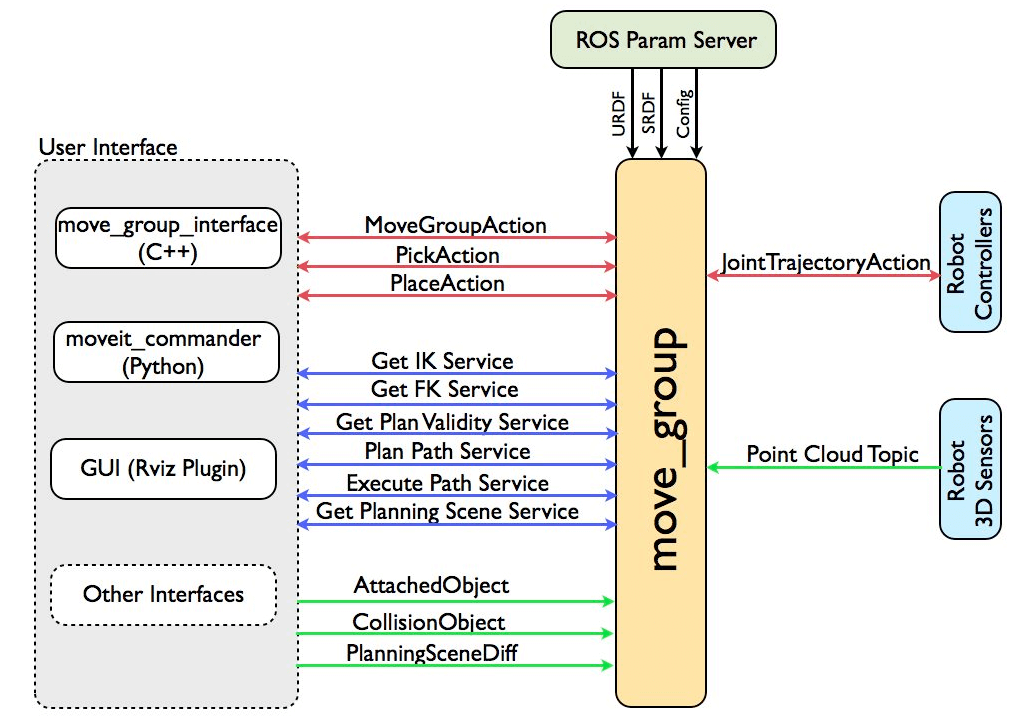
\includegraphics[width=15cm]{figs/moveit_arquitectura.png}
    \end{center}
    \caption{Relación de \textit{move\_group} con el resto del Firmware}
    \label{fig:arquitectura_moveit}
\end{figure}\ 

Primeramente, es necesario crear tener \textit{launcher}, esto es, una herramienta que se utiliza para iniciar, configurar, gestionar y desplegar 
nodos. Para ello, se va a hacer uso del ya existente implementado un fichero llamado \textit{real\_robot\_GUI.launch.py} que se encarga de lanzar una ventana de Rviz con todo lo necesario 
para controlar de forma gráfica el robot, además de lanzar el nodo \textit{move\_group}, entre otros. Este launcher se ha creado a partir 
de la demo que se crea automaticamente al generar el paquete. Era necesario modificar este para eliminar el controlador falso que se desplegaba 
para hacer pensar a moveit que habia un robot conectado y poder realizar la simulación. Esto es así ya que se desea poder utilizar el robot 
real. Se puede lanzar este launcher con:
\begin{verbatim}
    ros2 launch g_arm_moveit real_robot_GUI.launch.py
\end{verbatim}

Por simplicidad y robusted, se ha optado por utilizar un controlador virtual de ROS Control e imitar el estado de los joints en el robot 
real. Esto permite desacoplar toda la lógica de control de nuestro robot.



\newpage
\subsubsection{Interpretando tal}

\section{Pruebas}
En esta sección se pone a prueba los aspectos técnicos que determinan el desempeño y la fiabilidad del brazo robot. 
características.

\subsection{Estabilidad y vibración}
Este tipo de pruebas determinan como el movimiento del mismo afecta en su estabilidad y estructura. Además se determina el nivel de 
vibraciones no deseadas que puedan afectar su precisión y desempeño.
\begin{table}[H]
\begin{center}
\begin{tabular}{|c|c|}
\hline
\textbf{Parámetro} & \textbf{Valor} \\
\hline
Capacidad de carga máxima (completamente extendido) & $\pm9mm$\\
Capacidad de carga máxima (medio extendido) & $\pm9mm$\\
Capacidad de carga máxima (contraido) & $\pm9mm$\\
Capacidad de carga máxima (operativa) & $\pm9mm$\\
\hline
\end{tabular}
\caption{Evaluación de la estabilidad}
\label{cuadro:evaluacion_estabilidad}
\end{center}
\end{table}

\subsection{Capacidad de carga}
En este tipo de pruebas se evalua la capacidad del brazo a la hora de levantar diferentes pesos. De esta manera se puede determinar 
el límite de carga del brazo y verificar si puede manejar objetos de manera segura y eficiente sin perder capacidades.
\begin{table}[H]
\begin{center}
\begin{tabular}{|c|c|}
\hline
\textbf{Parámetro} & \textbf{Valor} \\
\hline
Capacidad de carga máxima (completamente extendido) & \SI{10}{\kilo\gram} \\
Capacidad de carga máxima (medio extendido) & \SI{10}{\gram} \\
Capacidad de carga máxima (contraido) & \SI{10}{\gram} \\
Capacidad de carga máxima (operativa) & \SI{10}{\gram} \\
\hline
\end{tabular}
\caption{Evaluación de la capacidad de carga}
\label{cuadro:evaluacion_carga}
\end{center}
\end{table}

Tablita de como afecta el peso a la precisión y demás

\subsection{Velocidad y tiempo de respuesta}
Es importante realizar este tipo de pruebas para evaluar las distintas velocidades que es capaz de manejar el brazo en la ejecución 
de diferentes movimientos. Además, se puede evaluar la capacidad del brazo para responder rápidamente a comandos y ajustar su 
velocidad rápidamente.

\begin{table}[H]
\begin{center}
\begin{tabular}{|c|c|}
\hline
\textbf{Parámetro} & \textbf{Valor} \\
\hline
Velocidad máxima & \SI{10}{\meter\per\second}\\
Aceleración máxima & \SI{10}{\meter\per\second}\\
Tiempo de respuesta (señal de la herramienta) & \SI{35}{\milli\second} \\
Tiempo de respuesta (movimiento del brazo) & \SI{35}{\milli\second} \\
\hline
\end{tabular}
\caption{Evaluación de la velocidad y tiempo de respuesta}
\label{cuadro:evaluacion_velocidad}
\end{center}
\end{table}

\subsection{Exactitud y repetitividad} 
Se procede a realiza pruebas para evaluar la precisión del brazo robot en la ejecución de movimientos y la repetibilidad 
de estos movimientos. Se mide la desviación del brazo robot en comparación con las coordenadas objetivo y verificar si 
es capaz de alcanzar de manera consistente los mismos puntos en un cierto número de intentos.


